% !TEX encoding = UTF-8 Unicode

\documentclass[a4paper]{report}
\usepackage[francais]{babel}
\usepackage[T1]{fontenc}
\usepackage[utf8]{inputenc}
\usepackage{geometry}
\usepackage{graphicx}
\usepackage[colorlinks=true]{hyperref}
\hypersetup{urlcolor=blue,linkcolor=red,colorlinks=false} 
\usepackage{algorithm,algorithmic}
\usepackage{listings}
\usepackage{amssymb}
\usepackage{setspace}
\usepackage{listings}
\usepackage{lscape}
\usepackage{amsmath}

\usepackage{tikz}
\usetikzlibrary{trees}
\usetikzlibrary{arrows,shapes}

\usepackage[normalsize]{subfigure}
\usepackage{verbatim}

\pagestyle{headings}
\thispagestyle{empty}
\geometry{a4paper,twoside,left=2.5cm,right=2.5cm,marginparwidth=1.2cm,marginparsep=3mm,top=2.5cm,bottom=2.5cm}


\begin{document}

\large
\setlength{\parskip}{5mm plus2mm minus2mm}
\lstset{language=C, showstringspaces=false, numbers=left, numberstyle=\tiny, tabsize=4}



\tikzstyle{vertex}=[circle,fill=black!25,minimum size=20pt,inner sep=0pt]
\tikzstyle{edge} = [draw,thick,-]
\tikzstyle{tree edge} = [draw, thick,->,red!75]
\tikzstyle{queue edge} = [draw,thick,->,blue!50]
\tikzstyle{cross} = [path picture={ \draw[black](path picture bounding box.south east) -- (path picture bounding box.north west) (path picture bounding box.south west) -- (path picture bounding box.north east);}]


\pgfdeclarelayer{background}
\pgfsetlayers{background,main}

 
{\setlength{\parindent}{0cm}
Chloé DESDOUITS \hfill M2 Informatique 2012\\
William DYCE \\
Thibaut MARMIN \\
Clément SIPIETER 
}
\vfill
{\centering \Huge \bfseries L'évolution informatique conduit-elle à une régression intellectuelle ?\par}
\vfill
Université Montpellier 2 \hfill  Épistémologie de l'informatique

\tableofcontents
\thispagestyle{empty}
\pagenumbering{arabic}


% !TEX encoding = UTF-8 Unicode
% !TEX root = rapport.tex

\chapter{Introduction}\label{intro}





% !TEX encoding = UTF-8 Unicode
% !TEX root = rapport.tex

\chapter{Constat sur l'état actuel des impacts psychologique / neurobiologie de l'informatique sur l'être humain}\label{neurobio}



% !TEX encoding = UTF-8 Unicode
% !TEX root = rapport.tex

\chapter{L'historique des techniques d'apprentissage et de communication peut-il expliquer l'évolution des comportements ?}\label{historique}



% !TEX encoding = UTF-8 Unicode
% !TEX root = rapport.tex

\chapter{Quelles sont les initiatives mises en place pour contrer le phénomène de débilisation des individus par l'informatique}\label{initiatives_actuelles}

\section{Initiatives des pouvoirs publics}

\subsection{Mesures des pouvoirs publics français}

\subsubsection{opérations "portables" visant à l'accès du plus grand nombre à l'informatique}
\cite{portables35}
\cite{portables60}
\cite{portables40}

\subsubsection{Mesures en faveur de la prise en main de l'outil informatique}
\cite{b2i_c2i}
\cite{b2i}
\cite{isn}
    


\subsection{Mesures des pouvoirs publics internationaux}
Forum mondial sur l’éducation \cite{educ_forum}
Les TIC au service de l’éducation \cite{tics}
Un regard sur la trajectoire de l’informatique éducative au Brésil \cite{peixoto2006regard}
Willem J. PELGRUM, Arian T. SCHIPPER, "Indicators of computer integration in education" \cite{pelgrum1993indicators}



% !TEX encoding = UTF-8 Unicode
% !TEX root = rapport.tex

\section{Initiatives des acteurs privés}



% !TEX encoding = UTF-8 Unicode
% !TEX root = rapport.tex

\chapter{Quelles peuvent être les solutions adaptées pour endiguer le phénomène ?}\label{solutions}



% !TEX encoding = UTF-8 Unicode
% !TEX root = rapport.tex

\part{Conclusion}\label{conclu}

\chapter*{L'effet dominos}
Nous avons vu lors de la première partie que de tous temps les sociétés ont une certaine réticence aux innovations technologiques. Au niveau du système éducatif et de l'arrivée des ordinateurs personnels, cela a rapidement créé un décalage entre la société et les écoles. Ce décalage occasionne de nombreux troubles, comme la difficulté à l'insertion professionnelle, de nombreux échecs scolaires (distraction des élèves), voir de tragiques évènements comme le suicide de jeunes pris aux piège de la diffusion de contenus intimes via internet (voir seconde partie).

\begin{figure}[H]
  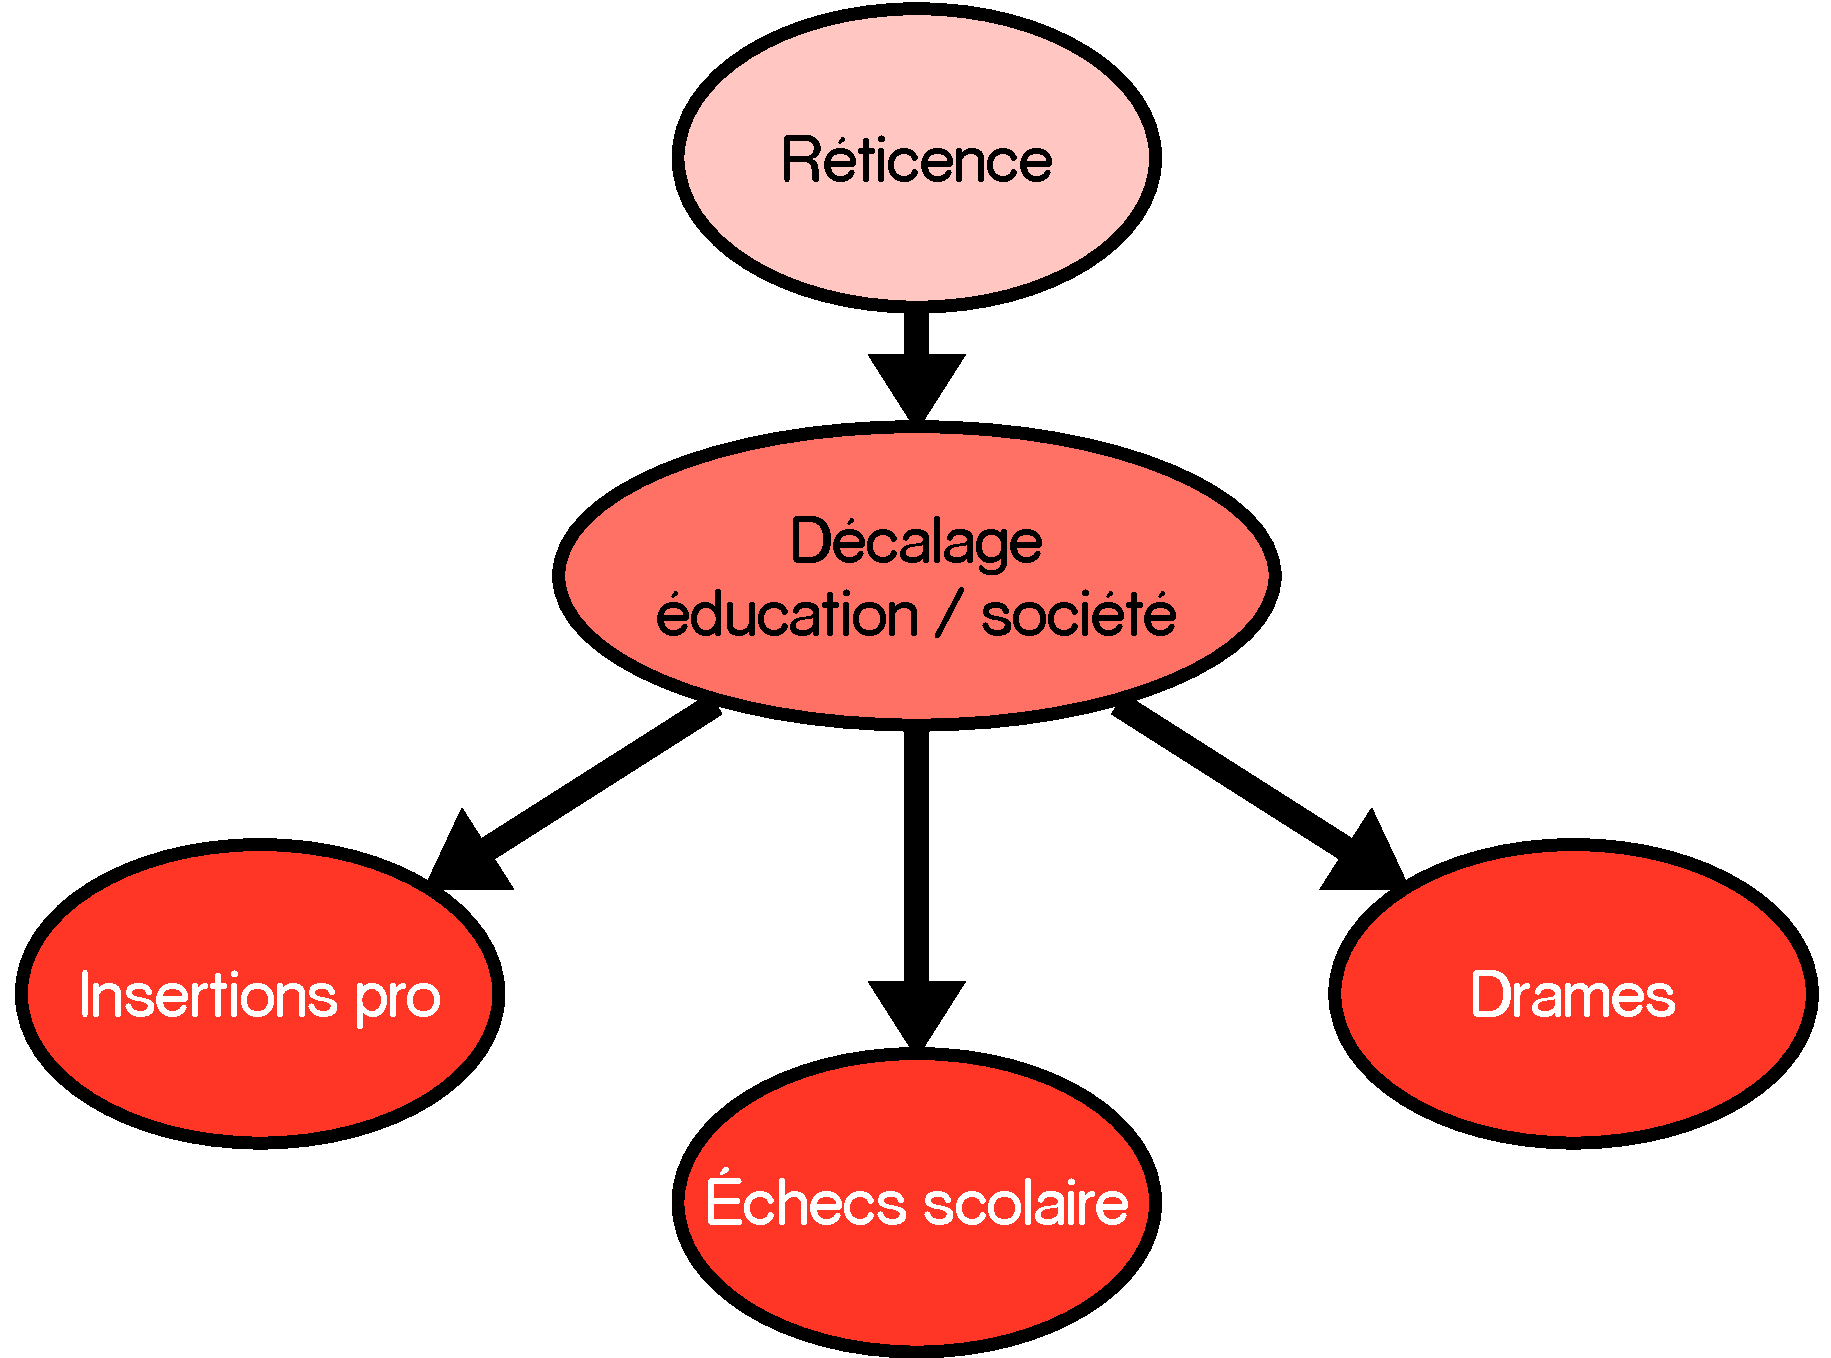
\includegraphics[width=\textwidth]{../resources/illustrations/ccl}
  \caption{Effet dominos causé par la réticence du système éducatif à l'intégration des \gls{ntic}.}
\end{figure}

\chapter*{Concrètement}
Comment pourrions-nous améliorer le système éducatif concrètement ? Nous avons tenu à rappeler quelques points, certainement classés du plus simple au plus complexe à mettre en œuvre.

\begin{description}
  \item[Projets vs. Problèmes] : un élève ne sera naturellement pas impliqué dans la résolution d'un problème dont la correction est donnée 15 minutes plus tard. Ici nous proposons de regrouper et d'inclure ces problèmes dans des projets globaux, effectués en groupes pour favoriser les interactions, et cela sur plusieurs jours (de deux jours à une semaine).
  \item[Multi-niveaux] : bien que le découpage des classes par âge n'ait pas vraiment de sens face à un découpage par centres d'intérêts ou de compétences, nous comprenons bien difficulté de gestion administrative. C'est pourquoi nous proposons, tout en conservant cette répartition par âge, de ne plus voir les différents niveaux comme des frontières, afin de pouvoir organiser des projet mixtes multi-niveaux. Cela permettrait un enrichissement mutuel, notamment les plus jeunes apportent une vision nouvelle sur certains problèmes, et les plus âgés auront tendance à prendre le rôle d'encadrant et d'enseignant.
  \item[Multi-disciplinaires] : beaucoup de sujets regroupent en fait de nombreux domaines. L'idée de briser les frontières entre les disciplines permettrait la réalisation de projets extrêmement intéressants au travers de sujets transversaux en mêlant plusieurs enseignements voir sections ou cursus universitaires.
  \item[Concret avant Abstrait] : idée essentielle et facile à appliquer qui découle directement de la philosophie du contructionnisme : toujours confronter l'élève à la problématique avant de lui enseigner des problèmes concrets.
  \item[Investissement sur l'avenir] : le constat est simple, le système éducatif devrait faire comme le font les grandes entreprises en investissant sur l'avenir. Il serait certainement plus raisonnable d'effectuer des recherches pour développer de nouvelles méthodes d'éducation plutôt que de renouveler les parcs informatiques.
\end{description}

\chapter*{Vers les neurosciences\ldots}
Avant de clôturer ce rapport, nous souhaitons souligner le fait que d'autre méthodes d'apprentissages existent, notamment basées sur les neurosciences. En effet de réels progrès ont eu lieu dans ce domaine ces dix dernières années, ce qui a permis, grâces aux connaissances acquises sur le fonctionnement du cerveau, de mettre en place des exercices adaptés \cite{neurosup}. Particulièrement, nous savons que la réalisation d'un résumé en fin de cours, de préférence sous la forme d'une carte mentale favorise grandement la mémorisation des leçons.

\begin{figure}[H]
  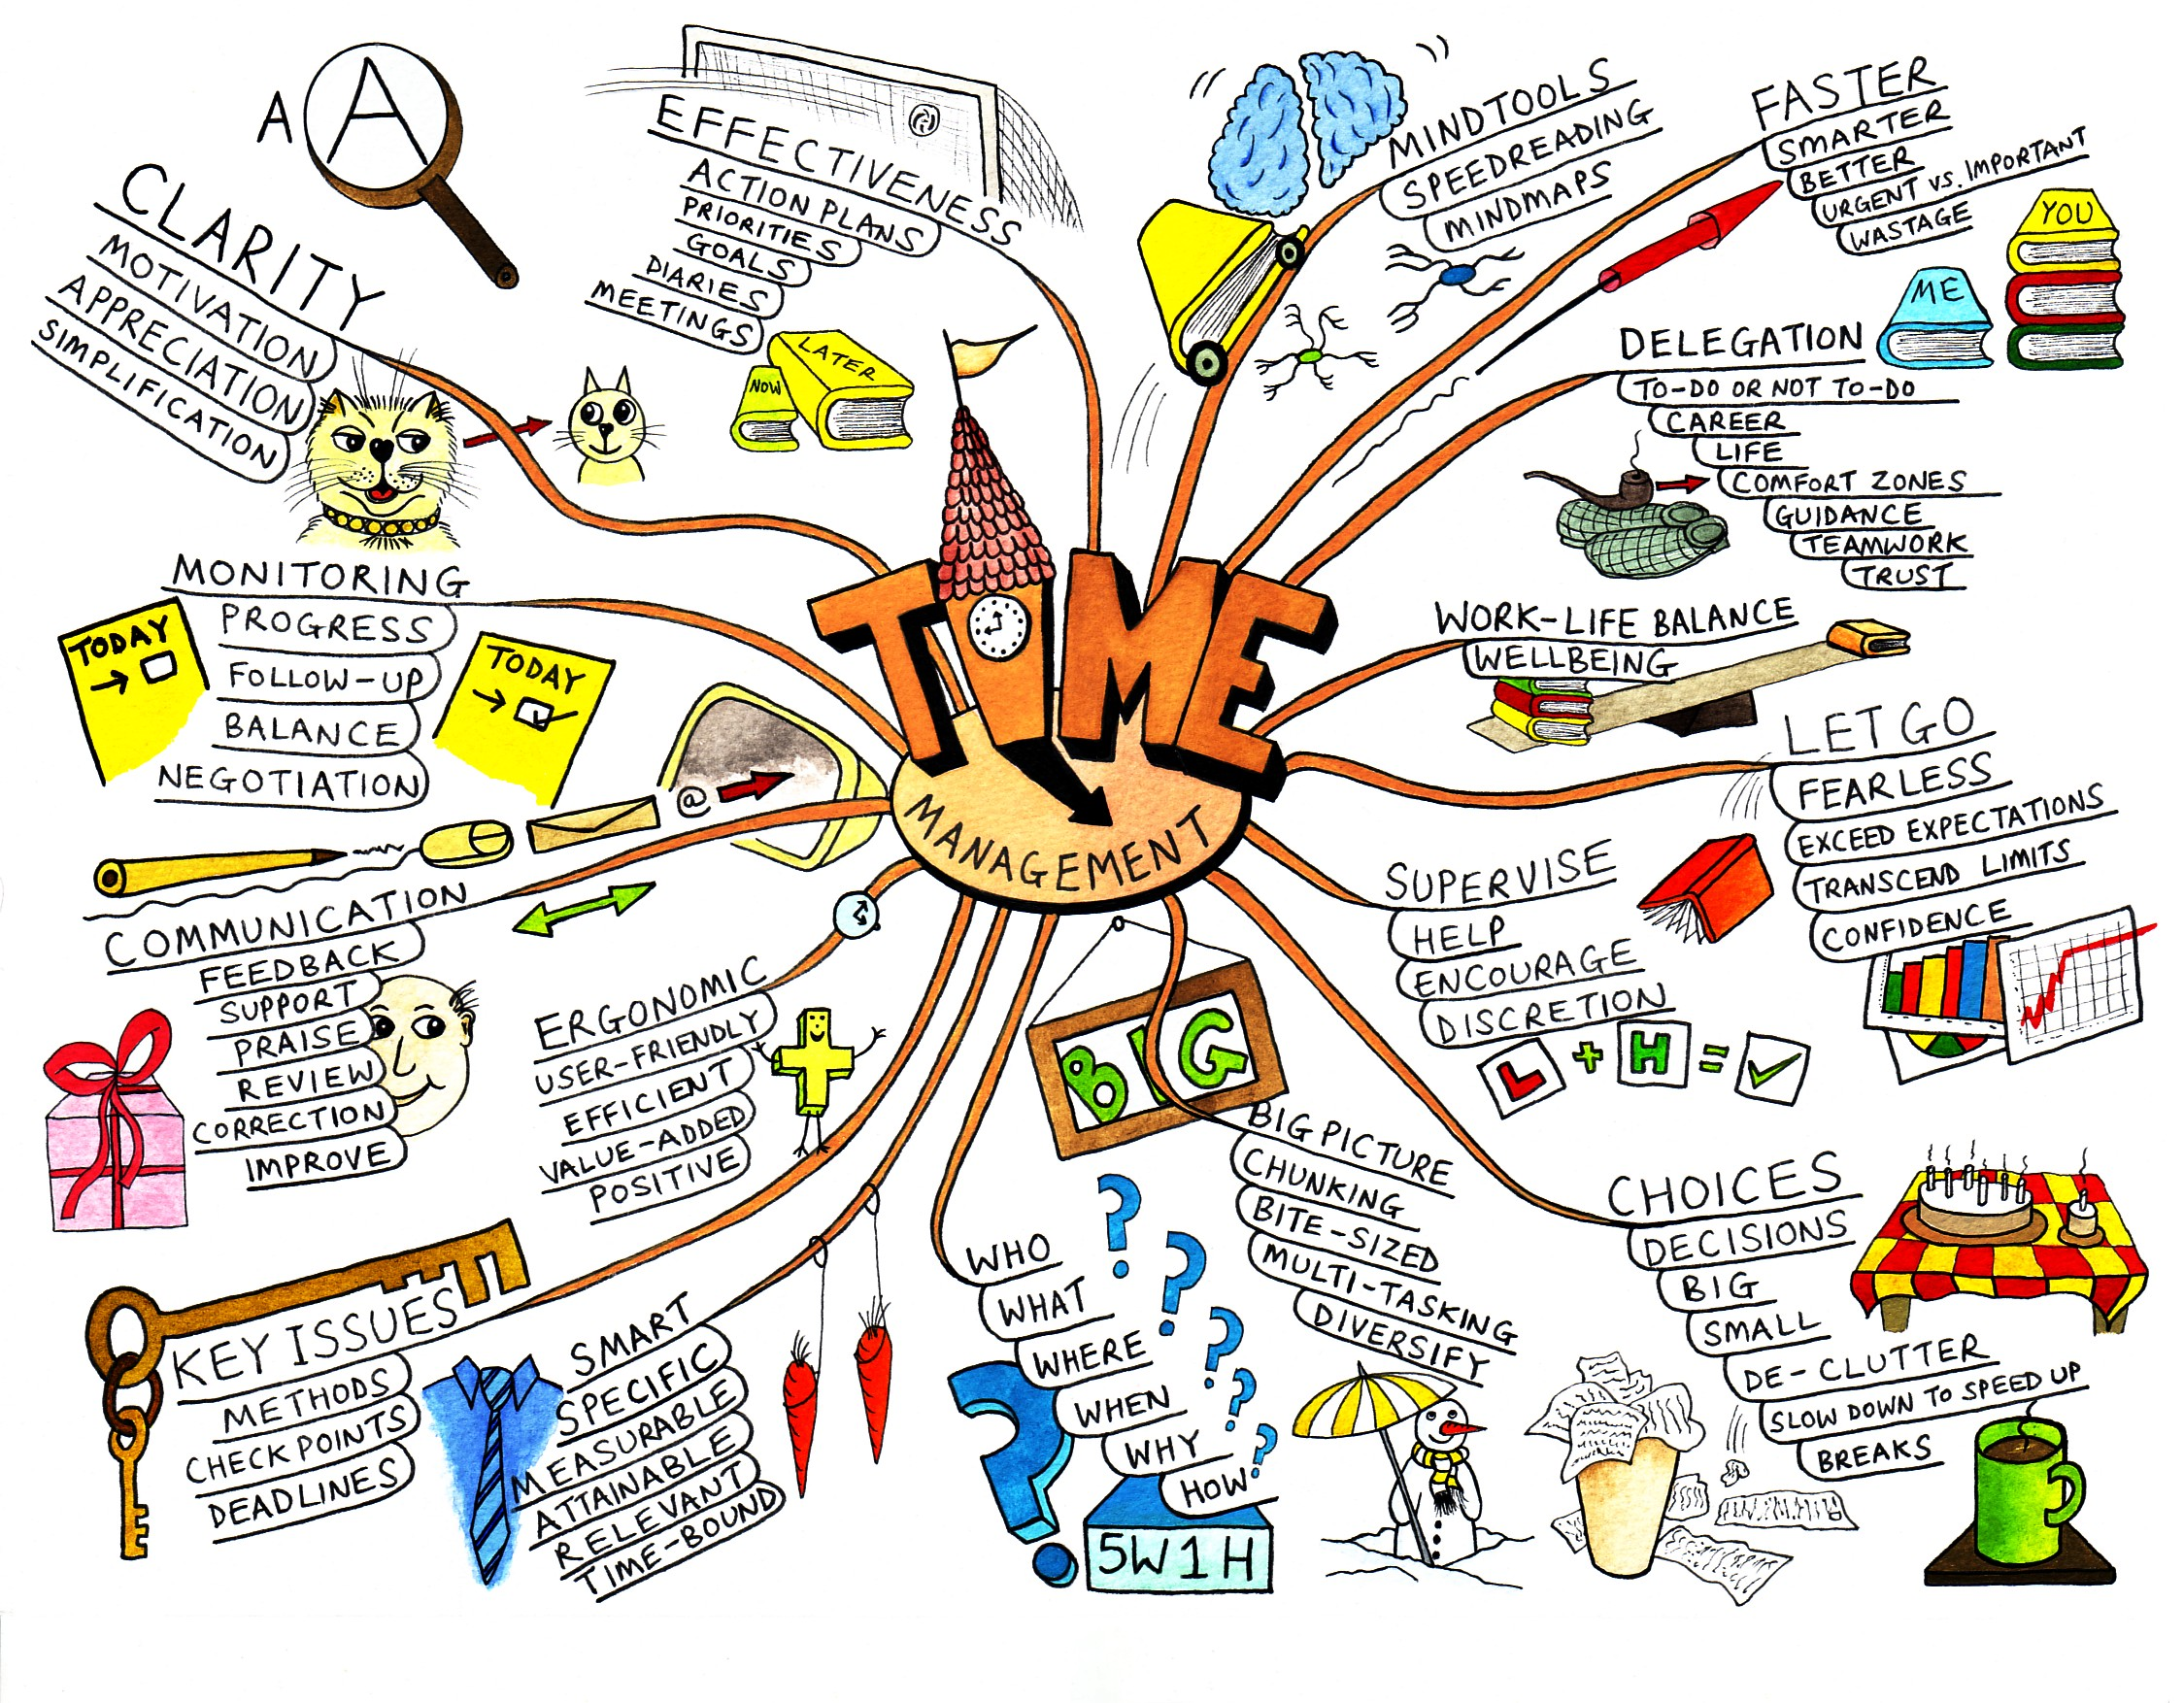
\includegraphics[width=\textwidth]{../resources/illustrations/mindmap}
  \caption{Exemple de carte mentale.}
\end{figure}

Ajoutons tout de même que les méthodes d'apprentissage qui résultent des résultats obtenus dans le domaine des neurosciences n'entrent pas forcément en opposition avec le constructionnisme. Nous somme convaincu par le fait que rester ouvert aux différentes sphères de la recherche permettra de développer de meilleurs approches concernant l'apprentissage et le système éducatif en général.

\bibliographystyle{plain}
\bibliography{Bib}

\vfill
{\raggedleft Réalisé avec \LaTeX{} \par}

\end{document}
